% !TeX spellcheck = en_GB
\documentclass{article}


\usepackage{fancyhdr} % Required for custom headers
\usepackage{lastpage} % Required to determine the last page for the footer
\usepackage{extramarks} % Required for headers and footers
\usepackage[usenames,dvipsnames]{color} % Required for custom colors
\usepackage{graphicx} % Required to insert images
\usepackage{subcaption}
\usepackage{courier} % Required for the courier font
\usepackage{enumerate}
\usepackage{amssymb}
\usepackage{amsmath}
\usepackage{array}
\usepackage{alphalph}
\usepackage{pdflscape}
\usepackage{afterpage}
\usepackage{capt-of}% or use the larger `caption` package
\usepackage{float}
\usepackage{titlesec}
\usepackage{algorithm}
\usepackage[noend]{algpseudocode}

%----------------------------------------------------------------------------------------
% Page setup information

\renewcommand*{\thesubfigure}{%
	\alphalph{\value{subfigure}}%
}%
% !TeX spellcheck = en_GB

% Margins
\topmargin=-0.45in
\evensidemargin=0in
\oddsidemargin=0in
\textwidth=6.5in
\textheight=9.0in
\headsep=0.25in

\linespread{1.1} % Line spacing

% Set up the header and footer
\pagestyle{fancy}
\chead{\compName: \docTitle} % Top center head
\rhead{\firstxmark} % Top right header
\lfoot{\lastxmark} % Bottom left footer
\cfoot{} % Bottom center footer
\rfoot{Page\ \thepage\ of\ \protect\pageref{LastPage}} % Bottom right footer
\renewcommand\headrulewidth{0.4pt} % Size of the header rule
\renewcommand\footrulewidth{0.4pt} % Size of the footer rule

\setlength\parindent{0pt} % Removes all indentation from paragraphs

% Set up section header formatting
\titleformat{\section}{\large \bfseries}{\thesection.}{0.5em}{}
% \titlespacing{\section}{0pt}{15pt}{6pt} % Uncomment to adjust paragraph spacing after section headings

% ----------------------------------------------------------------
% Title stuff
\newcommand{\docTitle}{Embedded Subsystem}
\newcommand{\compName}{CAN-RGX}
\newcommand{\authorName}{Hanzhen Lin, Tyler Gamvrelis, Twesh Upadhyaya}

\title{
	\vspace{2in}
	\textmd{\textbf{\compName:\ \docTitle}}\\
	\vspace{0.1in}
	\vspace{3in}
}

\author{\textbf{\authorName}}

% ----------------------------------------------------------------
\begin{document}
\maketitle
\clearpage

%
%
%
%

\section*{Introduction} \label{intro}
This document describes the embedded subsystem onboard team ``FAM"'s (fluids affect by magnetism) experiment for the Canadian Reduced Gravity Experiment Design Challenge.

\clearpage

%
%
%
%

% ----------------------------------------------------------------
\tableofcontents
\clearpage


%
%
%
%

\section{Overview} \label{overview}
The embedded subsystem is responsible for acquiring data from sensors, using this data to initiate control sequences, and streaming data to the onboard PC. The sensors are as follows:

\begin{enumerate}
	\item MPU9250: 3-axis accelerometer, gyroscope, and magnetometer, 1 in quantity
	\item MC9701A: analog temperature sensor
\end{enumerate}

The systems to which control signals will be asserted are as follows:

\begin{enumerate}
	\item DRV8871: H-bridge, 6 in quantity
	\item TEC: thermoelectric cooler, 2 in quantity
\end{enumerate}

The proceeding sections will describe each of these in more detail, and subsequently, their integration will be described.

\clearpage

%
%
%
%

\section{MPU9250} \label{MPU}
As the MPU9250 measures acceleration, it is capable of automatically triggering the experiment through software once the acceleration magnitude is below a certain threshold. It can also detect other events of interest throughout the flight. The aircraft detected these events according to the following algorithm, where:

\begin{enumerate}
	\item $w_y$ is the rate of change of the pitch of the aircraft about the y-axis (also called \textit{angular rate}). Note that pitch is the angle between the nose of the aircraft and the horizon in degrees per second.
	
	\item $a_z$ is the vertical acceleration of the aircraft. \textbf{Note that $a_z > 0$ implies the aircraft is accelerating downward}.
\end{enumerate}

\begin{algorithm}
	\caption{Algorithm used by plane for triggering flight events}
	\label{alg:flightEventsPlane}
	\begin{algorithmic}[1]
		\Procedure{FlightEventsPlane}{}
			\State{Measure $w_y$ and $a_y$}
			\If{$w_y > 2.5$ AND $a_z < -14.715 \ (1.5G)$}
				\State \Return{Transition from Straight and level to Pull Up}
				
			\ElsIf{$w_y < 0$ AND $a_z > -0.981 \ (0.1G)$}
				% If aircraft is changing its pitch to be more downward and is accelerating upward at less than 0.1G...
				\State \Return{Transition from Pull-up to Reduced Gravity}
				
			\ElsIf{$w_y > 0$ AND $a_z < -0.981 \ (0.1G)$}
				% If aircraft is changing its pitch to be more upward and is accelerating upward at more than 0.1G...
				\State \Return{Transition from Reduced Gravity to Pull-Out}
				
			\Else
				\State \Return{No flight event}
				
			\EndIf
		\EndProcedure
	\end{algorithmic}
\end{algorithm}

The algorithm actually implemented on the microcontroller was much more simple in nature and only detected reduced gravity events. It is shown in Algorithm~\ref{alg:flightEventsMicro}.

\begin{algorithm}
	\caption{Algorithm used in microcontroller for detecting reduced gravity}
	\label{alg:flightEventsMicro}
	\begin{algorithmic}[1]
		\Procedure{FlightEventsMicro}{}
		\State{Measure $a_z$, $a_y$, $a_x$}
		\If{$||a|| < 0.981$}
		\State \Return{Reduced gravity}
		
		\Else
		\State \Return{No flight event}
		
		\EndIf
		\EndProcedure
	\end{algorithmic}
\end{algorithm}


\textbf{Note:} It was suggested that a manual mechanism be provided to trigger the experiment in addition to the automated software protocol
\newline
\newline

The MPU9250 is also used to measure the magnetic field generated by the electromagnet. This allows the magnetic field to be generated to its maximum possible value while maintaining safety limits, and also is important for analysis of the experimental results.
\newline
\newline
At a minimum, the MPU9250 must be used to measure the following:
\begin{itemize}
	\item $a_x$, $a_y$, $a_z$ (16 bits, full-scale range $\pm 2g$)
	\item $H_x$, $H_y$, $H_z$ (14 bits each, full-scale range $\pm 4912 \ [uT]$)
\end{itemize}

Note that these full-scale ranges were the defaults and also the most suitable since they provided the highest resolution for the window of interest. Note that the full-scale range of 4912 for $H_i$ was taken from page 50 of the register map, while the datasheet specified 4800.
\newline
\newline
Also, functions were written that can retrieve angular rate data, for example, $w_y$ (16 bits, full-scale range $\pm 250 \ [\deg/s]$). This was done to provide flexibility for the triggering algorithm.
\newline
\newline

Due to the importance of the readings from the MPU9250, it was decided that the motion processing algorithms should be run at a high rate, about 500 [Hz]. Also, note that the MPU9250 features offset registers that can be user-programmed to eliminate dc offsets. It also features an integrated digital low-pass filter whose bandwidth can be set using the \texttt{DLPF\_CFG} and \texttt{A\_DLFPCFG} for the gyroscope and accelerometer, respectively. Note that lower bandwidth comes at the cost of increased delay, on the order of milliseconds. Because of this, usage of the LPF was not deemed useful for this application, although this was not explored in-depth.

\begin{figure}[!ht]
	\centering
	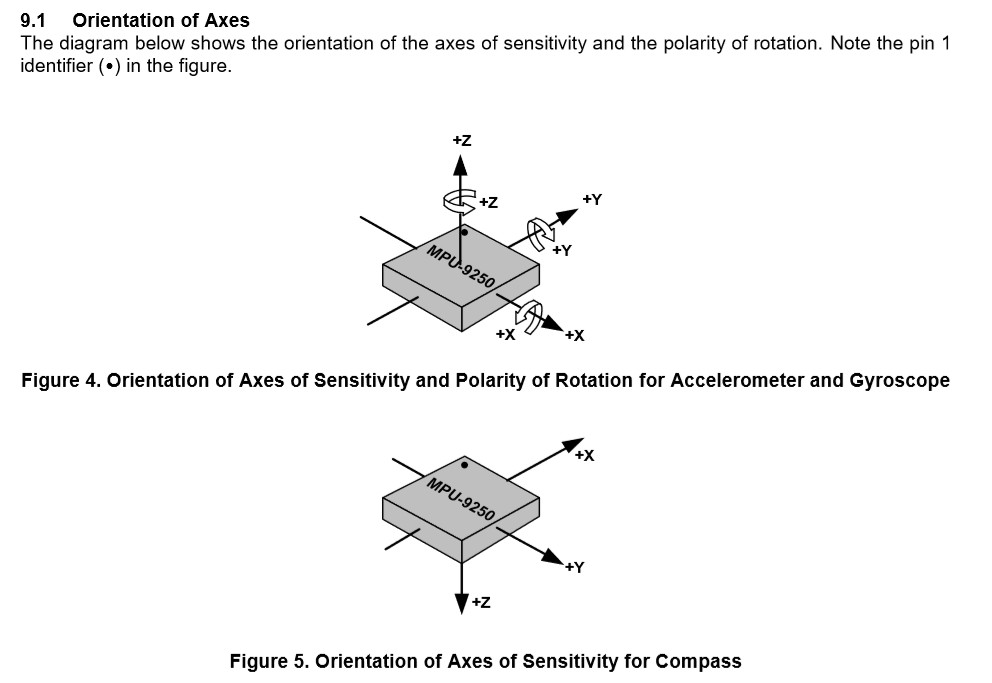
\includegraphics[width=0.75\textwidth]{images/MPU9250_axisOrientation}
	\label{MPUAxisOrientation}
	\caption{Orientation of axes for MPU9250 data (page 38 of datasheet).}
\end{figure}


\begin{figure}[!ht]
	\centering
	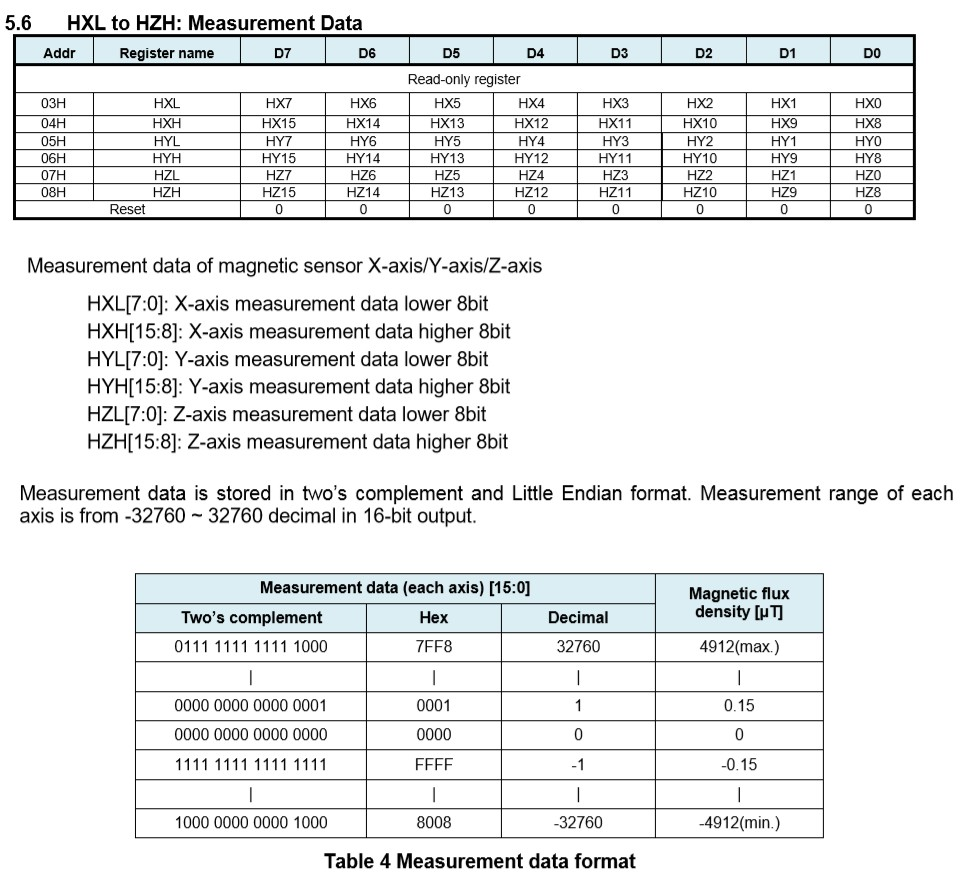
\includegraphics[width=0.75\textwidth]{images/MPU9250_magnetometerRegs}
	\label{MPUMagRegs}
	\caption{Magnetometer register map and corresponding scales from page 50 of the register map.}
\end{figure}

\clearpage

Implementation details will now be described. To begin, it was decided that the $400 \ [kHz]$ I\textsuperscript{2}C bus would be used to transfer data to and from the sensor. However, there is no reason why this could not be changed to $1 \ [MHz]$ or $20 \ [MHz]$ SPI. The code related to the MPU9250 was split into $2$ parts:
\begin{enumerate}
	\item start-up routine, where the peripheral is initialized
	
	\item data-gathering and processing routine used during the experiment
\end{enumerate}

\textit{Start-up routine}
\newline
Initializing the MPU9250 consists of initializing two different devices, the accelerometer and gyroscope (device 1) and the magnetometer (device 2). Although these are integrated as 1 physical package, under the hood they remain distinct. Consequently, the accelerometer and gyroscope have a slave address of 0x68, and the magnetometer has a slave address of 0x0C. Now, there are two important points to make before continuing:

\begin{itemize}
	\item The magnetometer must be controlled \textit{by proxy} through the accelerometer and gyroscope. Essentially, the accelerometer and gyroscope have the ability to control \textit{slave devices}, and in the MPU9250, ``slave 0" is directly connected to the magnetometer.
	
	\item ST's HAL libraries for I\textsuperscript{2}C require the slave address to be shifted 1 bit to the left in calls to I2C functions. This only affects calls to the accelerometer and gyroscope, since as was just noted above, the magnetometer is ultimately controlled by these.
\end{itemize} 

This will become more clear shortly.
\newline
\newline
The start-up routine is called prior to starting the scheduler. This way, more primitive I/O interfaces (i.e. polled I/O) can be used to avoid complexity. Also, it increases the probability that nothing will interrupt the start-up sequence since there is no context switching.
\newline
First, all the fields in the global MPU9250 handle, called \texttt{myMPU9250}, are initialized to $-1.0$. Next, the WHO\_AM\_I register is read from the accelerometer and gyroscope. This is a read-only register that should always return 0x71, so this check basically ensures that the correct device is connected to the bus. Next, the accelerometer and gyroscope are configured as follows:

\begin{enumerate}
	\item The best available clock source is selected
	
	\item The I\textsuperscript{2}C master interface module is enabled
	
	\item The I\textsuperscript{2}C module is set to $400 \ [kHz]$ bus speed
	
	\item The accelerometer and gyroscope are set to ON
	
	\item I\textsuperscript{2}C bypass is enabled. This is critically important for getting the magnetometer to work
\end{enumerate}

Next, the magnetometer is configured as follows:

\begin{enumerate}
	\item Check the ID of the magnetometer
	
	\item Reset the magnetometer and delay $10 \ [ms]$
	
	\item Enable continuous measurement
\end{enumerate}

If the startup routine makes it to the end, it returns $1$. Otherwise, a unique negative integer is returned whose value depends on the cause of failure.
\newline
\newline

\textit{Data-gathering and processing routine}
\newline
This routine runs after the scheduler is started. It begins by calling \texttt{vTaskDelayUntil()} such that it runs every 2 milliseconds ($500 \ [Hz]$ refresh rate). Next, the accelerometer and magnetometer are read. Then, the acceleration is checked for the experiment event conditions as per Algorithm~\ref{alg:flightEventsMicro}.
\newline
\newline
The total number of bytes required for these transfers is as follows. Note that write transactions are 2 bytes, while read transactions are 2 bytes plus the number of bytes read back
\begin{itemize}
	\item Get accelerometer data for $a_z$: 1 write transaction (accelerometer data address) + 2 bytes returned for the data = 4 bytes
	
	\item Get accelerometer data for $a_y$: 4 bytes
	
	\item Get accelerometer data for $a_x$: 4 bytes
	
	\item Get magnetometer data: 1 call to \texttt{magnetometerRead()} = 3 write transactions (I2C\_SLV0\_ADDR, I2C\_SLV0\_REG, I2C\_SLV0\_CTRL) + 1 read transaction of 6 bytes for magnetometer data (starting from EXT\_SENS\_DATA\_00) = 3 * 2 + 2 + 6 = 14 bytes
\end{itemize}

The total number of bytes transferred to get all the data required for the experiment is thus:

\begin{equation}
4 \times 3 + 14 = 26 \ bytes
\end{equation}

So the lower limit on the time required for the data transfer is:

\begin{equation}
26 * 8 / 400 \times 10^3 = 520 \ [\mu s]
\end{equation}

The acquisition of the accelerometer and gyroscope data is accomplished using DMA. First, \texttt{HAL\_I2C\_Mem\_Read\_DMA} is called to initiate the data transfers, and then \texttt{xSemaphoreTake(semMPU9250Handle, portMAX\_DELAY)} is executed. This second line forces the MPU9250 thread to block (i.e. not run) until the semaphore \texttt{semMPU9250Handle} is given from the I2C callback, \texttt{HAL\_I2C\_MemRxCpltCallback}. For reading from the magnetometer, interrupt-driven writes were used along with DMA-based reads. Interrupt-driven writes were used instead of DMA-based writes because the callback for DMA-based writes was not working properly.

\clearpage

%
%
%
%

\section{MC9701A} \label{tempsensor}
The temperature sensor is used to monitor the temperature of the electromagnet.

Can have up to 6 of these with the current board
TODO: Details
\clearpage

%
%
%
%

\section{DRV8871} \label{hbridge}
The H-bridges are used to generate magnetic fields of various strengths in the coils surrounding the fluid cell, and to generate various heat gradients using the TECs. PWM is used in both cases.
\clearpage

%
%
%
%

\section{TEC} \label{18B20}
The TEC plates are used to supply heat and cooling to the fluid.

Power data should be acquired at about 500 Hz
\clearpage

%
%
%
%

\section{Integration} \label{integration}
The aforementioned components were integrated using a STM32F446RE microcontroller on a Nucleo-F446RE development board.

\subsection{Data Logging}
Data from all sensors were logged and sent to the onboard PC over a 230400 [symbol/s] UART channel. The UART function used DMA and a semaphore to optimize CPU usage.


Note that the symbol rate of 230400 [symbols/s] corresponded to an upper limit on the byte rate of 
$$B_t = 23.04 \ [bytes/s]$$
This is seen in \ref{eq:byterate}. Note that there are 10 bits transmitted per byte since for each byte transferred (8 bits), there is also a start bit and a stop bit.

\begin{equation}\label{eq:byterate}
\frac{230400 \text{ [symbols]}}{\text{[s]}}
\times 
\frac{1 \text{ [bit \ transmitted]}}{\text{symbol}}
\times
\frac{1 \text{ [bytes]}}{10 \text{ [bits transmitted]}}
\times
\frac{1 \text{ [s]}}{1000 \text{ [ms]}}
=
23.04 \text{ [bytes/ms]}
\end{equation}


The packet format was as follows:

\begin{table}[!ht]
	\centering
	\begin{tabular}{ | m{4cm} | m{2cm} | m{2cm} | m{2cm}| m{1cm}| m{2cm}| m{2cm}|  } 
		\hline
		Parameter & Data Type & Size (bytes) & Offset (bytes) & Units & Range & Positive Sign Convention \\
		\hline
		Dummy bytes & uint8\_t & 2 & 0 & na & na & na \\
		\hline
		Tick stamp & uint32\_t & 4 & 2 & $ms$ & [0, $2^{32}-1$] & na \\ 
		\hline
		Acceleration X & float & 4 & 6 & $m/s^2$ & $\pm 2g$ & TODO \\ 
		\hline
		Acceleration Y & float & 4 & 10 & $m/s^2$ & $\pm 2g$ & TODO \\ 
		\hline
		Acceleration Z & float & 4 & 14 & $m/s^2$ & $\pm 2g$ & TODO \\ 
		\hline
		Magnetic flux density X & float & 4 & 18 & $\mu T$ & $\pm 4912$ & TODO \\ 
		\hline
		Magnetic flux density Y & float & 4 & 22 & $\mu T$ & $\pm 4912$ & TODO \\ 
		\hline
		Magnetic flux density Z & float & 4 & 26 & $\mu T$ & $\pm 4912$ & TODO \\ 
		\hline
		Magnet 1 power & uint16\_t & 2 & 30 & TODO & TODO & TODO \\ 
		\hline
		Magnet 1 power & uint16\_t & 2 & 32 & TODO & TODO & TODO \\ 
		\hline
	    TEC 1 duty cycle & uint16\_t & 2 & 34 & \% & $[0, 100]$ & TODO \\ 
		\hline
		TEC 1 duty cycle & uint16\_t & 2 & 36 & \% & $[0, 100]$ & TODO \\ 
		\hline
		Thermocouple 1 & uint16\_t & 2 & 38 & TODO & TODO & TODO \\ 
		\hline
		Thermocouple 2 & uint16\_t & 2 & 40 & TODO & TODO & TODO \\ 
		\hline
		Thermocouple 3 & uint16\_t & 2 & 42 & TODO & TODO & TODO \\ 
		\hline
		Thermocouple 4 & uint16\_t & 2 & 44 & TODO & TODO & TODO \\ 
		\hline
		Thermocouple 5 & uint16\_t & 2 & 46 & TODO & TODO & TODO \\ 
		\hline
		Thermocouple 6 & uint16\_t & 2 & 48 & TODO & TODO & TODO \\ 
		\hline
		
	\end{tabular}
	\caption{Form of packet to PC. Total length: 50 bytes}
	\label{tab:PCPacketFormat}
\end{table}

Additionally, the aircraft provided its own data as a UDP packet on port 5124, which could be read by the onboard PC so long as it had an IP address of 132.246.192.[25..50]. A breakdown of the packet can be found in ``NRC Nav Packet.xlsx".
\clearpage

% ----------------------------------------------------------------
\end{document}
